\documentclass{aastex62}   	% use "amsart" instead of "article" for AMSLaTeX format
\usepackage{graphicx}				% Use pdf, png, jpg, or eps§ with pdflatex; use eps in DVI mode
								% TeX will automatically convert eps --> pdf in pdflatex		
\usepackage{amssymb}
\usepackage{natbib}
\usepackage{grffile}
\usepackage{textcase}
%SetFonts

%SetFonts

\begin{document}

\title{Testing Gravity using Type Ia Supernovae Discovered by LSST}
\author[0000-0001-6315-8743]{A.~G.~Kim}
\affiliation{    Physics Division, Lawrence Berkeley National Laboratory, 
    1 Cyclotron Road, Berkeley, CA, 94720}
\author{S.~BenZvi}
\affiliation{Department of Physics and Astronomy, University of Rochester, Rochester, NY 14627, USA}
\author{C.~Harper}
\affiliation{    Physics Division, Lawrence Berkeley National Laboratory, 
    1 Cyclotron Road, Berkeley, CA, 94720}
\author{D.~Huterer}
\affiliation{Department of Physics, University of Michigan, 450 Church Street, Ann
Arbor, MI 48109, USA }
\author{C.~Ju}
\affiliation{    Physics Division, Lawrence Berkeley National Laboratory, 
    1 Cyclotron Road, Berkeley, CA, 94720}

\author{others}

%\date{}							% Activate to display a given date or no date

\begin{abstract}
ZTF today and LSST in the upcoming decade will increase the number of identified  $z<0.3$ Type~Ia supernovae (SNe~Ia)  from the hundreds to the
hundreds of thousands.  The increase in the number density of SNe~Ia, in parallel with improvements in the standardization of
their absolute magnitudes, now make them competitive probes of the growth of structure.  The peculiar velocity power spectrum
is sensitive to $f\sigma_8$,
the product of the linear growth and amplitude of density perturbations.  Cross-correlation with synergistic galaxy surveys further constrains $f \sigma_8$ and the galaxy bias. 
Thus, in the next decade the peculiar velocities of
SNe~Ia will provide the growth of structure  in the local $z<0.3$ Universe as a powerful test of General Relativity and other models of gravity.
\end{abstract}

\section{Connection between Type Ia Supernovae Correlations and Gravity}

The growth of structure depends on the expansion history of the Universe, the nature and density of its contents, and gravity. 
It is therefore a powerful probe of cosmology and dark energy.  Growth of structure can be measured from the baryonic structures
in the Universe and from the peculiar velocities of test masses therein.
Peculiar velocities are the motions, on top of the cosmological expansion, caused by the gravitational attraction
and repulsion of densitiy inhomogeneities in the Universe.  The peculiar velocity of an object with a known absolute magnitude
is determined from its observer magnitude and redshift. For a given a background cosmology, the observed magnitude provides
an estimate of the cosmological redshift, the peculiar velocity is then the difference between the cosmological and observer redshifts.

Baryonic structures and peculiar velocities  provide a measurement of the combination $fD$.  $D$ is the ``linear growth factor'' that
gives the overall amplitude of  overdensities, and the ``linear growth rate''
$$f \equiv \frac{d\ln{D}}{d\ln{a}}$$ is how that amplitude changes with redshift.  General Relativity predicts
$f \approx \Omega_M^\gamma$ (with $D$ determined accordingly) with $\gamma=0.55$, whereas other gravity models can be similarly described
with different values of $\gamma$
\citep{2007APh....28..481L}.  The growth of structure, through the measurement of $fD$, provides a test of General Relativity and breaks degeneracies
between gravitational and dark energy models that explain the accelerating expansion of the Universe.
The parameter $\sigma_8$, the  standard deviation of overdensities in 8$h^{-1}$Mpc spheres, is 
commonly used in place of $D$ to normalize the
overall amplitude of  overdensities, so the standard parameterization used by the community is $f\sigma_8$.

Baryonic structures are sensitive to $f\sigma_8$ through redshift space distortions (RSD), 
which gives the combination $(b + f \mu^2)\sigma_8$ where $b$ is the bias between the tracer and dark matter
and $\mu$ gives the angular separation.  Correlations between peculiar velocities are sensitive to  $f\sigma_8 (H_0 d_L)^{-1}$.
Although the velocities may be measured off of biased tracers, the tracers' dynamics are driven by all mass (including dark matter) and are so bias-free.
As
mentioned earlier, peculiar velocities are measured relative to the background cosmological expansion that
leads to the dependence on $H_0 d_L$. 
Baryonic structures and peculiar velocities within the same volume are induced by the same overdensities  making their cross-correlation 
insensitive to sample variance \citep{2007PhRvL..99h1301G}: galaxy and peculiar velocity surveys provide synergistic constraints more powerful
than their naive sum.

The probative power of a specific peculiar-velocity tracer primarily depends on its number density and the precision to which its absolute magnitudes are known.
The current generation of peculiar velocity studies use $10^3-10^5$ galaxies with Fundamental Plane and Tully-Fisher distances \citep{2008AJ....135.1738M, 2014MNRAS.445.2677S,
2016AJ....152...50T}.  These galaxies have absolute magnitude uncertainties of $\sim 0.4$~mag. 
Next generation surveys WALLABY \citep{2008ExA....22..151J} and TAIPAN \citep{2017PASA...34...47D} are designed to increase these sample size by an order of magnitude
over half the sky to a depth of $z=0.1$.


The current sample of SNe~Ia has a low number density compared to Fundamental Plane and Tully-Fisher galaxies.
Nevertheless, their low intrinsic-magnitude uncertainties can 
can provide peculiar velocities (expressed equivalently as peculiar magnitudes)
of their host galaxies \citep{2006PhRvD..73l3526H,2011ApJ...741...67D}.  Existing SN~Ia samples
have been used to test and ultimately find spatial correlations in peculiar velocities that may be attributed to the growth of structure
\citep{2008MNRAS.389L..47A,2015JCAP...12..033H, 2017JCAP...05..015H}.
However, the signal-to-noise is currently insufficient to perform a meaningful test of GR.

Two advances in the upcoming decade will make SNe~Ia  important probes of $f\sigma_8$.
First, the precision of SN~Ia distances can be improved.  The commonly-used empirical 2-parameter SED model yields $\sigma_M \gtrsim 0.12$~mag absolute magnitude
dispersion.  However, SNe transmit more information than just the light-curve shape and single color used in current SN models.
Recent studies indicate that with the right data, SNe absolute
magnitudes can be calibrated to $\sigma_M \lesssim 0.08$ mag \citep[see e.g.][]{2012MNRAS.425.1007B, 2015ApJ...815...58F}.
One such SN is worth $\gtrsim 25$ galaxies with 0.4~mag absolute magnitude uncertainty.
Secondly,  ZTF today and LSST in the upcoming decade will increase the number of identified  $z<0.3$ Type~Ia supernovae (SNe~Ia)  from the hundreds to the
hundreds of thousands.  This is a sample size comparable to the number of galaxies projected by WALLABY and TAIPAN.

The precision in  $f\sigma_8$ derived from the baseline WFD ten-year SN~Ia discoveries has been projected by \citet{2017ApJ...847..128H},
from both their RSD and peculiar velocities.
The results are summarized in Table~\ref{tab:howlett}, where a 5\% distance uncertainty is assumed for each supernova.
SNe~Ia alone can provide a $2\%$ measurement of $f\sigma_8$ at $z<0.3$ redshifts lower than where galaxy, cluster, and Ly$\alpha$
RSD measurements are sensitive.  A joint galaxy RSD and SN peculiar velocity will be even more powerful.
{\bf Add a SN PV + DESI-like BGS column and/or a PV-only column with Cullan's code? }

% Requires the booktabs if the memoir class is not being used
\begin{table}
   \centering
   %\topcaption{Table captions are better up top} % requires the topcapt package
   \begin{tabular}{@{} lccc @{}} % Column formatting, @{} suppresses leading/trailing space
	\hline
	Redshift & RSD & RSD + PV & cumulative\\ \hline
      $0.00<z<0.05$   & 66.3 & 13.9 & 13.9\\
     $0.05<z<0.10$            & 24.6     &  7.3 & 6.5\\
     $0.10<z<0.15$      & 14.8  & 5.8 & 4.3\\
     $0.15<z<0.20$      & 10.6  & 5.0 & 3.3\\
      $0.20<z<0.25$     & 8.3  & 4.4 & 2.6\\
     $0.25<z<0.30$  & 6.8  &  4.0 & 2.2\\
      \hline
   \end{tabular}
   \caption{Projected percent uncertainties in $f\sigma_8$ from a 10-year LSST SN survey with 5\% distance uncertainties from
   \citet{2017ApJ...847..128H}. RSD is from clustering, and RSD~+~PV is from joint clustering and peculiar velocities.
   The cumulative column shows the effective uncertainty from combining the redshift and all other shallower redshift bins.}
   \label{tab:howlett}
\end{table}

The projected precisions for LSST-discovered SNe~Ia have a number of interesting features. 
Despite the significant gain in volume and numbers of supernovae, the $f\sigma_8$ uncertainty in increasing redshift bins asymptotes such that 
there is little benefit in going beyond
$z=0.3$.
The constraining power on  $f\sigma_8$ 
comes primarily from peculiar velocities
at $z<0.2$, but are dominated by RSD by $z=0.3$.
It turns out that for $z>0.1$, the volume is sufficiently large that the LSST sample is not yet sample variance limited.

\section{Important Elements in Designing a Supernova Survey to Measure $\MakeLowercase{f}\sigma_8$}
\citet{2017ApJ...847..128H} perform their analysis in Fourier space, 
where the Fisher information matrix of a random Gaussian field with mean zero and covariance $C(k)$ parameterized by $\lambda$ is
\begin{equation}
F_{ij} = \frac{V}{2}\int \frac{d^3k}{(2\pi)^3} \text{Tr}\left[ C^{-1} \frac{\partial C}{\partial \lambda_i} C^{-1}
\frac{\partial C}{\partial \lambda_j} \right],
\end{equation}
where the covariance for the velocity-velocity correlation
\begin{equation}
C = P_{vv}(k) + \frac{\sigma^2}{n}
\label{cov:eq}
\end{equation}
is dependent on the power spectrum, noise in the velocity measurement, and the density of velocity probes
\citep{2017MNRAS.464.2517H}.  
The primary dependence on the growth of structure is through
\begin{equation}
\frac{\partial C}{\partial \lambda} = \frac{\partial P_{vv}}{\partial \lambda} = \text{constant}
\end{equation}
for the parameter choice
$\lambda=(f\sigma_8)^2$.  In the sample-variance limit, $F_{\lambda \lambda} \propto V$ whereas in the shot noise limit $F_{\lambda \lambda} \propto V n^2 \sigma^{-4}$.


The survey parameters that determine parameter precision are the volume $V$, which
in turn can be parameterized by the survey solid angle $\Omega$ and the redshift depth $z_{max}$ ; the number density of sources $n$; and the intrinsic
magnitude dispersion $\sigma_M$, where magnitude and velocity dispersions are related by $\sigma_{M} = \frac{5}{\ln{10}} \frac{1+z}{z} \sigma$.
LSST is expected to discover all $z<0.3$ SNe~Ia before maximum light in its active Wide Fast Deep (WFD) survey area.
Equating LSST discovery with having a meaningful peculiar velocity, $n$ is thus a non-tunable parameter.




For surveys of fixed depth, the variance of $f\sigma_8$ 
in the sample-variance limit  
is inversely proportional to the survey solid-angle $\Omega$, whereas
in the shot-noise limit the variance is inversely proportional to $\Omega n^2 \propto N^2/\Omega$, where $n$ is the number density,
and $N$ is the total number of supernovae.  




\subsection{Solid Angle}

The variance in $f\sigma_8$ is proportional to solid angle $\Omega$ given a fixed redshift depth and  $\sigma^2_M/n$.  The baseline
LSST survey covers 18,000 sq.~deg, at $-75 \lesssim \delta \lesssim15$ avoiding the Galactic plane.  Larger solid-angle coverage for $z<0.3$ SN~Ia searches, beyond
the LSST baseline, benefits peculiar-velocity science.  Complementary northern-hemisphere surveys and LSST-expanded or independent
coverage of the southern equatorial pole, could double
the sky coverage and halve the variance in $f\sigma_8$.

\subsection{Intrinsic Magnitude Dispersion}
The quality of supernova follow-up is an important factor in how well a peculiar-velocity survey can measure $f\sigma_8$.
Supplemental non-LSST data can access SN models that yield lower intrinsic-magnitude dispersion and systematic errors.
LSST SN~Ia light curves from the WFD survey, with their relatively poor sampling, plus a spectroscopic redshift
 can give $\sigma_M \sim 0.15$~mag.
 Non-LSST follow-up including infrared data \citep{2012MNRAS.425.1007B} or spectrophotometry at peak brightness
 \citep{2015ApJ...815...58F} are projected to give
$\sigma_M \lesssim 0.08$~mag.
Uncertainties in $f\sigma_8$ depend on $\sigma^2_M/n$ so the improvement between 0.08 and 0.15~mag dispersions is equivalent to a factor of 3.52
 in number density, or in survey duration. 
While LSST data can be used to obtain photometric redshifts from host galaxies and supernova light curves, the spectroscopic
redshifts needed for precise host-galaxy peculiar velocities require other resources.

LSST can be taken to be a SN~Ia discovery plus light-curve builder, or a discovery machine only.  The former comes with a simplified follow-up program of typing
and/or redshift collection but with higher intrinsic magnitude dispersion.  The latter requires additional follow-up resources to gather more information per supernova to
lower the intrinsic magnitude dispersion.

The nominal observing strategy will obtain photometry every couple of days rotating through the 6 $grizy$ bands.  Although SNe have good
overall sampling, the per-band light curves are poorly sampled.


\appendix
\section{Reanalysis in Configuration Space}

This Appendix describes a new analysis used to project precisions on $f\sigma_8$ using peculiar velocities derived from SNe~Ia.
This analysis may or may not be useful for the Decadal Survey White Paper, but will be helpful for LSST planning.
While there have been a number of articles on the subject,
our analysis brings a higher level of fidelity than sought previously.  We simulate SNe~Ia hosted by galaxies in a mock galaxy
catalog. The numbers of SNe are sufficiently small to allow fast evaluations of the likelihood, which enable the determination of parameter
posteriors using MCMC on reasonable computing timescales.   We can use our machinery to 
compare different survey parameters, such as redshift depth, total numbers of supernovae, non-uniform spatial density,
solid angle/survey geometry, and SN~Ia intrinsic magnitude dispersion.
Adding the cross-correlation between galaxy-count and peculiar-velocity surveys is active work, so we can
quantify the suppression of sample variance achieved when considering matter-densities and velocities 
within the same volume \citep{2007PhRvL..99h1301G}.

\section{Simulated Data}
The cosmoDC2 (v1.0) covering 706 sq.~deg is used\footnote{We previously used
Buzzard (v1.6) galaxy catalog is used, but it was found to give peculiar velocities inconsistent with general relativity.  As we will see,
cosmoDC2 (v1.0) is consistent with GR. }. 
The catalog is based on a Flat $\Lambda$CDM model with $H_0=71$~km~s$^{-1}$,  $\Omega_M=0.265$, $\Omega_B=0.0448$, and
$\Omega_\nu=0$.
Each galaxy has its cosmological redshift, the $x$-, $y$-, $z$-components of its peculiar velocity from which
the radial peculiar velocity is determined, and its
star formation rate and stellar mass from which the
supernova rate of each host is determined using 
\citet{2012ApJ...755...61S}.   This host-based rate
underestimates the expected discovery based on the volumetric
rate of \citet{2010ApJ...713.1026D}.  The volumetric rate is more robust, so  we boost the SN production
by a factor 2.4 to get the 10-year volumetric rate expectation. The total number of simulated SNe 
is greater than the total number of possibly useful supernova discoveries, since most fields cannot be continuously monitored throughout the year
from most ground-based observatories.


Each supernova is assigned a magnitude based on the distance modulus of its cosmological
redshift plus a random term drawn from a Normal distribution $\sigma_M$, which for simplicity is the same for all supernovae and captures both
intrinsic magnitude dispersion and measurement uncertainty.  No other corrections are applied to the observed magnitude.  Dipole effects of the heliocentric
motion with respect to the CMB and of the galaxies with respect to the CMB  are ignored: referring to
\citet{2011ApJ...741...67D}, the effects in Eq.~18 are not included.  Including these effects are straightforward but is computationally expensive
and does not affect our conclusions.

We consider a maximum redshift of $z=0.2$ because over ten years the noise is not sample-variance dominated, meaning that the differential improvement
in the precision of
$f\sigma_8$ due to a lower-redshift supernova is greater than that due to a high-redshift supernova.  Following all LSST SNe~Ia below this redshift 
would likely saturate available follow-up resources.


\section{Analysis}
The analysis is  almost identical to that of \citet{2015JCAP...12..033H, 2017JCAP...05..015H}, except as noted later.  
The peculiar magnitude is given by 
\begin{equation}
\delta_m=(m - M) - \mu(z;H_0, \Omega_M, \Omega_\Lambda).
\label{data:eqn}
\end{equation}  We introduce one free parameter 
$\mathcal{M} = M - 5\log{H_0} + \text{const}$ and do not consider the other cosmological parameters, whose effects are relatively weak at low-redshift.


The peculiar magnitude correlation
function $\xi_{\delta m \delta m}$ \citep{2011ApJ...741...67D,2015JCAP...12..033H} expected from General Relativity acting on the CMB
matter density power spectrum is calculated using CAMB \citep{Lewis:2002ah}  assuming the same
cosmological parameters used for the cosmoDC2 catalog.  Our model for the data covariance
is
\begin{equation}
C_{ij} = A\xi_{\delta m \delta m}(\mathbf{r_i},\mathbf{r_j}) + \frac{\sigma_M^2}{N_i} \delta_{ij} + \sigma^2_{NL}(z_i;\sigma_{v})\delta_{ij},
\label{cov:eqn}
\end{equation}
where $N_i$ is the number of SNe~Ia in galaxy $i$ and $\sigma_M$ is the intrinsic SN magnitude dispersion.
The model is used to test General Relativity through deviations from $A=1$ but is not sensitive to deviations
from the linearized GR expectation of the shape of the power spectrum 
$\xi$.
Nevertheless, for
convenience we say that our model gives $f\sigma_8 = A (f\sigma_8)^{GR}$, where $(f\sigma_8)^{GR}$ is the expectation
from General Relativity. 
The final term includes extra magnitude dispersion produced by non-linear effects on velocity, parameterized with $\sigma_{v}$, such that
\begin{equation}
\sigma_{NL} = \frac{5}{\ln{10}} \frac{1+\bar{z}}{\bar{z}} \sigma_v,
\end{equation}
where $\bar{z}$ is the cosmological redshift of the host galaxy.
We note that the CAMB calculation of $\xi$ includes non-linear corrections, which actually may be a bad thing for peculiar velocities \citep{2015MNRAS.454.3920H}. 
Such subtleties are unimportant as \citet{2015JCAP...12..033H} find that their results are insensitive to whether non-linear corrections are or are not included.

For all analyses we remove supernovae below observed $z_{min}=0.01$ in order to
reduce errors made in the first-order transformation between velocity and
magnitude.  This cut removes a  small volume relative to the full survey.

The posterior of the parameters is sampled using emcee.  The likelihood is the Normal distribution with the data in Eq.~\ref{data:eqn} and
covariance matrix in Eq.~\ref{cov:eqn}.
The priors are positive and flat for $A$, flat for $M$, positive Cauchy(0.08, 0.5) for $\sigma_M$, and  positive Cauchy(0, 600 km~s$^{-1}$) for $\sigma_{v}$.

Direct tests of non-GR models for which Poisson's equation or the linear approximation
does not apply requires a model-dependent $\xi$.  We defer the analysis of such higher-fidelity models to later work. 

\section{Results of Subsets}

The  ston in $f\sigma_8$ is calculated for different subsamples of the simulated data.
For each subsample  the mean  and standard deviation, $(\bar{A}, \sigma_A$) of the amplitude parameter is
determined.  The ston in $f\sigma_8$ for the subsample is thus  $\bar{A} \sigma^{-1}_A$, and that for a 18,000 sq.~deg. survey  is approximated by
$\sqrt{18000/760}\bar{A}\sigma^{-1}_A$.  The effective constraining power of a single supernova in the subset is chracterized by 
 $\bar{A} \sigma^{-1}_A N_{gal}^{-0.5}$.

Different parameters describing the input simulated data define the subsamples, 
which are used to explore the range of possible survey strategies.   The varied parameters are the redshift range, $z_{max}$, intrinsic
magnitude dispersion, $\sigma_M$, and SN number density, $n = \phi n_{10}$, where $ n_{10}$ is the  10-year total number density.  In general a given point
of sky is not monitored over the full year.  
The fit posterior for one representative subsample, with input  $z_{max}=0.2$, $\sigma_M=0.08$, $\phi=0.65$, is shown in Figure~\ref{zmax:fig}.
For all subsamples, there is no evidence for non-convergence of the MCMC chains.  The parameter $\sigma_v$, not included in  \citet{2015JCAP...12..033H, 2017JCAP...05..015H},
is found to be consistent with zero, poorly constrained, and very weakly correlated with $A$.  Table~\ref{tab:subsets} gives the results for the different subsamples.

\begin{figure}
\centering
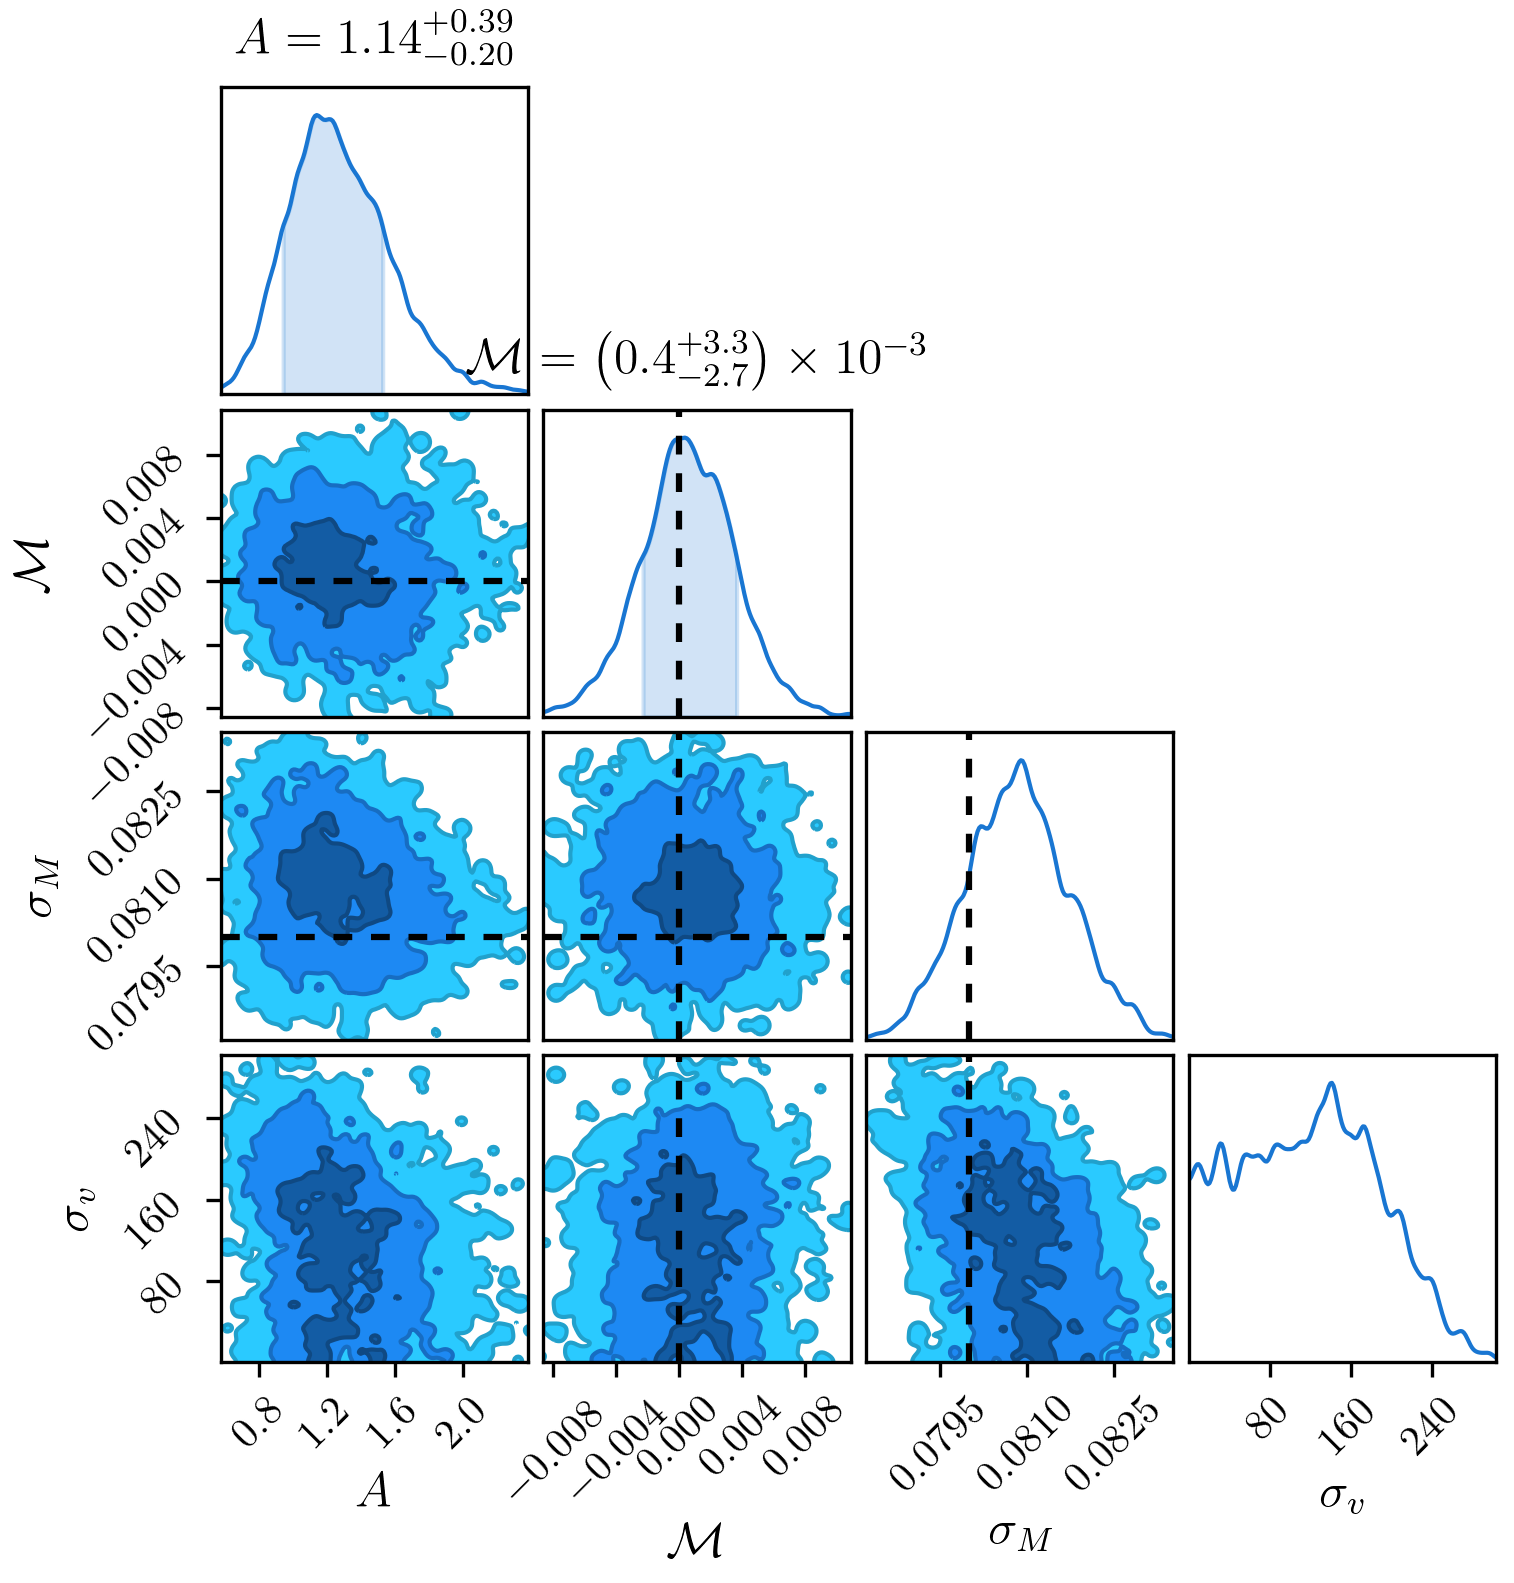
\includegraphics[width=0.5\textwidth]{../outcosmo/pvlist.0.08.1234.0.65.0.2.pkl.png}
\caption{Confidence regions for the model parameters.  $A=(f\sigma_8)/(f\sigma_8)_{GR}$, $\mathcal{M}$ is the supernova
absolute magnitude, $\sigma_M$ is the magnitude dispersion, and $\sigma_v$ is the non-linear contribution
to peculiar velocity.  This result is for the subset $z_{max}=0.2$, $\sigma_M=0.08$, $\phi=0.65$.  The dotted lines represent the inputs of the supernova
part of the simulation.
\label{zmax:fig}}
\end{figure}

\begin{table}
   \centering
   %\topcaption{Table captions are better up top} % requires the topcapt package
   \begin{tabular}{|ccc|ccccc|c|} % Column formatting, @{} suppresses leading/trailing space
   \hline
$z_{max}$ & $\phi$ & $\sigma_{M}$ & $N_{gal}$ & $\bar{A}$ & $\sigma_A$ & $\bar{A} \sigma_A^{-1} N_{gal}^{-0.5}$ & $\bar{A} \sigma_A^{-1} (18000/760)^{0.5}$&  STON $f\sigma_8$ \\
\hline
0.07 & 0.65 & 0.08 & 392 &   1.34 &   0.49 &  0.137 &  13.21 &  26.42\\
0.07 & 1.00 & 0.08 & 563 &   1.16 &   0.36 &  0.135 &  15.55 &  31.11\\
0.07 & 1.00 & 0.10 & 563 &   1.27 &   0.48 &  0.112 &  12.88 &  25.77\\
0.07 & 1.00 & 0.12 & 563 &   1.41 &   0.61 &  0.097 &  11.15 &  22.30\\
0.07 & 1.00 & 0.15 & 563 &   1.64 &   0.82 &  0.084 &   9.74 &  19.48\\
0.10 & 0.30 & 0.08 & 429 &   1.26 &   0.51 &  0.120 &  12.09 &  24.18\\
0.10 & 0.50 & 0.08 & 683 &   1.02 &   0.42 &  0.093 &  11.84 &  23.67\\
0.10 & 0.65 & 0.08 & 873 &   0.89 &   0.35 &  0.087 &  12.57 &  25.14\\
0.10 & 0.65 & 0.10 & 873 &   1.01 &   0.46 &  0.075 &  10.72 &  21.43\\
0.10 & 0.65 & 0.12 & 873 &   1.11 &   0.57 &  0.066 &   9.48 &  18.96\\
0.10 & 1.00 & 0.08 & 1294 &   0.91 &   0.28 &  0.091 &  15.96 &  31.91\\
0.10 & 1.00 & 0.10 & 1294 &   0.95 &   0.36 &  0.072 &  12.66 &  25.33\\
0.10 & 1.00 & 0.12 & 1294 &   1.04 &   0.43 &  0.067 &  11.71 &  23.41\\
0.15 & 0.30 & 0.08 & 1215 &   1.42 &   0.55 &  0.074 &  12.48 &  24.96\\
0.15 & 0.30 & 0.12 & 1215 &   1.97 &   0.92 &  0.061 &  10.36 &  20.73\\
0.15 & 0.50 & 0.08 & 1982 &   1.12 &   0.37 &  0.069 &  14.93 &  29.86\\
0.15 & 0.65 & 0.08 & 2541 &   1.15 &   0.33 &  0.070 &  17.05 &  34.11\\
0.15 & 0.65 & 0.10 & 2541 &   1.15 &   0.39 &  0.059 &  14.43 &  28.87\\
0.15 & 0.65 & 0.12 & 2541 &   1.30 &   0.51 &  0.051 &  12.42 &  24.83\\
0.15 & 1.00 & 0.08 & 3870 &   1.00 &   0.24 &  0.066 &  20.00 &  40.00\\
0.20 & 0.20 & 0.08 & 2021 &   1.66 &   0.59 &  0.062 &  13.61 &  27.21\\
0.20 & 0.30 & 0.08 & 3023 &   1.34 &   0.43 &  0.057 &  15.16 &  30.32\\
0.20 & 0.30 & 0.10 & 3023 &   1.40 &   0.54 &  0.047 &  12.68 &  25.37\\
0.20 & 0.30 & 0.12 & 3023 &   1.48 &   0.72 &  0.037 &   9.95 &  19.89\\
0.20 & 0.50 & 0.08 & 5015 &   1.13 &   0.30 &  0.054 &  18.54 &  37.07\\
0.20 & 0.65 & 0.08 & 6491 &   1.28 &   0.30 &  0.053 &  20.79 &  41.58\\
0.20 & 0.65 & 0.10 & 6491 &   1.24 &   0.34 &  0.046 &  17.95 &  35.89\\
0.20 & 0.65 & 0.12 & 6491 &   1.33 &   0.45 &  0.037 &  14.33 &  28.65\\
0.20 & 1.00 & 0.08 & 9901 &   1.18 &   0.23 &  0.050 &  24.38 &  48.77\\
0.20 & 1.00 & 0.10 & 9901 &   1.06 &   0.25 &  0.042 &  20.33 &  40.66\\
0.20 & 1.00 & 0.12 & 9901 &   1.09 &   0.28 &  0.040 &  19.13 &  38.26\\
    \hline
   \end{tabular}
   \caption{ston in $A$ or equivalently $f\sigma_8$ for surveys parameterized by the maximum redshift $z_{max}$,
   the fraction of total supernovae in 10 years ``fraction'', intrinsic magnitude dispersion $\sigma_{SN}$.  The number of galaxies
   $N_{gal}$, the signal $\bar{A}$ and its uncertainty $\sigma_A$ are for the cosmoDC2 (v1.0) 760 sq.~deg. volume only.
   The uncertainty ``per'' supernova is given by  $\sigma_A N_{gal}^{-0.5}$.  The ston, scaled to an LSST solid angle, is given as 
    $\bar{A} \sigma_A^{-1} (18000/760)^{0.5}$.
   \label{tab:subsets}}
\end{table}

In Fourier space, the data covariance is a combination of sample and shot noise (Eq.~\ref{cov:eq}).
In Figure~\ref{scaling:fig} the effective LSST ston is plotted as a function of input $n \sigma^{-2}_M$ for different $z_{max}$.
For all cases, the ston improves with larger $n \sigma^{-2}_M$ showing that the sample-variance limit has not been reached,
though the shallowing of the slopes for shallower surveys shows that it does contribute non-negligibly.
The fact that the ston is not constant indicates that not of the subsamples is sample-variance limited, though its non-linearity
indicates that it is non-negligible.


\begin{figure}
\centering
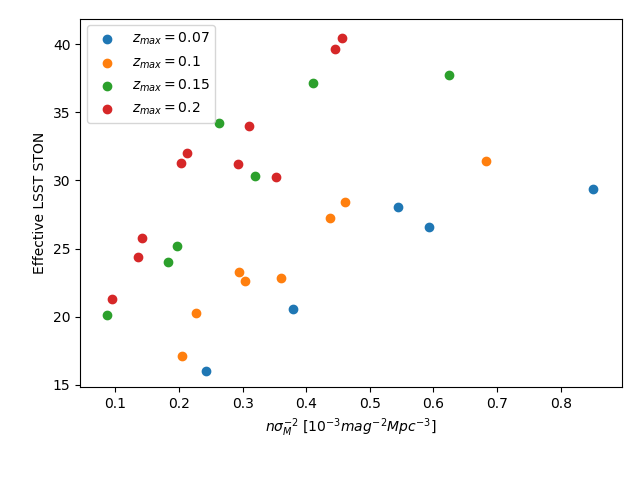
\includegraphics[width=0.5\textwidth]{../outcosmo/fracsnsig2_.png}
%\includegraphics[width=0.5\textwidth]{../outcosmo/zmax_.png}
\caption{ Effective LSST ston as a function of input  $n \sigma^{-2}_M$.  The points are color-coded for different $z_{max}$.
\label{scaling:fig}}
\end{figure}

A SN peculiar survey benefits from greater redshift depth $z_{max}$ due to the increase in volume and numbers of supernovae.  However,  for fixed magnitude uncertainty
peculiar-velocity uncertainties increase with redshift and the follow-up of fainter distant SNe requires more resources. 
Table~\ref{tab:subsets}
shows that the effective worth of each supernova ($\sigma_A N_{gal}^{-0.5}$) diminishes with increasing survey depth.
The table also shows that for $\sigma_M=0.08$~mag, the subsample with $z_{max}=0.1$ with 1294 supernovae yields a ston of 15.96, whereas
a sample with $z_{max}=0.2$ with 2021 supernovae has a lower ston of 13.61.  Within the range of surveys considered, a lower-redshift supernova
is more valuable than one at high redshift.  For both scientific and resource reasons, it is best to devote resources to the lowest possible redshifts.


$\phi \sim 0.65$ is an effective number density of discovered supernovae with light-curve coverage observed in 10 years


%We consider two different scenarios cutting at different redshift depths $z_{max}=0.1$ and  $z_{max}=0.15$.  All the objects in the first
%scenario are in the second scenario.  The results are shown in Fig.~\ref{zmax:fig}.  The points of interest are:
%\begin{itemize}
%\item There is a bias toward low $f\sigma_8$ for low-redshift ($z_{max}=0.1$).  Adding more supernova with increasing redshift
% decreases the bias  ($z_{max}=0.15$), and $A$ eventually approaches 1 ($z_{max}=0.2$ not shown).
% \item Based on the analysis of \citet{2017MNRAS.471.3135H}, I added an intrinsic velocity dispersion $\sigma_v$ (km~s$^{-1}$) due to non-linear effects.  This was not
% in Dragan's model.  My fit finds that this  dispersion is consistent with zero, not well constrained, and not strongly correlated with
% $A$.  The lack of covariance is consistent with Dragan's own tests.
% \item The fit intrinsic magnitude dispersion, on the other hand, is larger than the input $\sigma_M=0.08$ mag.  This  indicates that the catalogs
% contain 
% extra  velocity dispersion better attributed to intrinsic magnitude dispersion rather than correlated peculiar velocities.
%\end{itemize}


%\begin{figure}
%\includegraphics[width=0.5\textwidth]{../outcosmo/pvlist.0.08.1234.1.0.1.pkl.png}
%\includegraphics[width=0.5\textwidth]{../outcosmo/pvlist.0.08.1234.1.0.2.pkl.png}
%\caption{Confidence regions for the model parameters.  $A=(f\sigma_8)/(f\sigma_8)_{GR}$, $M$ is the supernova
%absolute magnitude, $\sigma_M$ is the magnitude dispersion, and $\sigma_v$ is the non-linear contribution
%to peculiar velocity.   The parameters for which I controlled the input, $M=0$ and $\sigma_M=0.08$~mag, are shown in dotted lines.
% Left: A survey truncated at $z_{max}=0.1$.  Right: A survey truncated at $z_{max}=0.2$.
%\label{zmax:fig}}
%\end{figure}
%

%
%\begin{itemize}
%\item Dragan: Is there some way that the formalism in your article breaks down at low-redshift?  I do remove very low-redshift objects at $z<0.01$,
%which I think is conservative.
% \item Risa/Joe: Is there any reasons for the Buzzard catalog to not capture correlated peculiar velocities on small scales (box size to large?) nor capture
% non-linear velocities?  (I don't know how to translate a mass resolution of 2.7e10 $M_{\odot}/h$ into a spatial resolution!)
%\end{itemize}

\bibliographystyle{aasjournal}
\bibliography{/Users/akim/Documents/alex}

\end{document}  